\chapter{Énols, énolates et aldolisation}\label{ch:b2:enolates-aldol}

Chaque fois qu'une cellule dégrade du glucose, une enzyme coupe un sucre phosphate à six carbones
en deux fragments à trois carbones~: c'est une \omterm{def:b2:enolates-aldol:aldol}{aldolisation} menée à l'envers. Menée dans le sens
direct, la même réaction réunit deux composés carbonylés en un seul, et c'est le moyen le plus
utilisé par les chimistes pour créer des liaisons carbone--carbone. Elle repose sur une propriété
que les chapitres précédents n'ont fait qu'effleurer~: les atomes d'hydrogène voisins d'un groupe
carbonyle sont acides, et en arracher un fait du carbone voisin du carbonyle un nucléophile.

\begin{recall}
Le volume de première année~: $\mathrm pK_a$ et réaction prépondérante, carbanions, contrôle
cinétique et thermodynamique, \omterm{def:b2:amines:nucleophilic-addition}{additions nucléophiles} sur les carbonyles, éliminations E1 et E2,
hydratation des alcynes (réarrangement d'un \omterm{def:b2:enolates-aldol:tautomerism}{énol}). \Cref{ch:b2:frontier-orbitals}~: \omterm{def:b2:frontier-orbitals:ambident}{nucléophiles
ambidents}. \Cref{ch:b2:acyl-substitution}~: esters et substitution acyle.
\end{recall}

\section{Tautomérie céto--énolique}

\begin{definition}[Tautomérie]\label{def:b2:enolates-aldol:tautomerism}
Les \emph{tautomères}\index{tautomeres@tautomères} sont des isomères qui se transforment l'un en
l'autre par déplacement d'un hydrogène et d'une double liaison. Dans la \emph{tautomérie
céto--énolique}\index{tautomerie ceto--enolique@tautomérie céto--énolique}, un composé carbonylé
portant un hydrogène sur le carbone voisin du carbonyle (la forme cétone) est en équilibre avec son
\emph{énol}\index{enol@énol}, un alcool porté par une double liaison \ce{C=C}.
\end{definition}

\begin{omfigure}
\setchemfig{atom sep=2em}
\schemestart
\chemfig{H_3C-C(=[2]O)-CH_3}
\arrow{<=>[\ce{H+} ou \ce{HO-}][catalyse]}[,2.2]
\chemfig{H_3C-C(-[2]OH)=CH_2}
\schemestop
\par\vspace{6pt}

{\small La propanone et son \omterm{def:b2:enolates-aldol:tautomerism}{énol}, le prop-1-én-2-ol. Un acide (protonation de l'oxygène du
carbonyle, puis perte d'un hydrogène $\alpha$) ou une base (arrachement d'un hydrogène $\alpha$, puis
protonation de l'oxygène) catalyse la transformation~; l'équilibre est très largement déplacé du
côté de la forme cétone.}
\end{omfigure}

\begin{proposition}[Teneur en énol]\label{prop:b2:enolates-aldol:enol-content}
Les aldéhydes et cétones simples ne contiennent que des traces d'\omterm{def:b2:enolates-aldol:tautomerism}{énol}~; les composés
1,3-dicarbonylés comme la pentane-2,4-dione en contiennent une forte proportion.
\end{proposition}

\begin{proof}[Argument]
Une liaison \ce{C=O} est plus forte qu'une liaison \ce{C=C} de davantage qu'une liaison \ce{O-H} n'est
plus faible qu'une liaison \ce{C-H}~: la forme cétone est favorisée. Dans un composé 1,3-dicarbonylé,
la double liaison de l'\omterm{def:b2:enolates-aldol:tautomerism}{énol} est conjuguée avec le second groupe carbonyle, et le \ce{OH} de l'\omterm{def:b2:enolates-aldol:tautomerism}{énol}
forme avec son oxygène une liaison hydrogène interne, dans un cycle à six atomes~: ces deux effets
stabilisent assez l'\omterm{def:b2:enolates-aldol:tautomerism}{énol} pour en faire une forme majoritaire.
\end{proof}

Comme l'\omterm{def:b2:enolates-aldol:tautomerism}{énol} est plan au niveau de sa liaison \ce{C=C}, un stéréocentre situé sur le carbone $\alpha$
est perdu chaque fois que l'\omterm{def:b2:enolates-aldol:tautomerism}{énol} se forme~: une cétone optiquement active portant un stéréocentre
voisin de son carbonyle se racémise en milieu acide ou basique.

\section{Énolates}

\begin{definition}[Énolates]\label{def:b2:enolates-aldol:enolate}
Le \emph{carbone $\alpha$}\index{carbone alpha@carbone $\alpha$} d'un composé carbonylé est le carbone
lié au carbone du carbonyle~; ses hydrogènes sont les \emph{hydrogènes $\alpha$}\index{hydrogene alpha@hydrogène $\alpha$}.
En arracher un donne un \emph{ion énolate}\index{ion enolate@ion énolate}, dont la
charge négative est partagée entre le carbone $\alpha$ et l'oxygène.
\end{definition}

\begin{proposition}[Acidité des hydrogènes $\alpha$]\label{prop:b2:enolates-aldol:alpha-acidity}
Les hydrogènes $\alpha$ sont bien plus acides que les liaisons \ce{C-H} ordinaires, parce que l'\omterm{def:b2:enolates-aldol:enolate}{énolate}
est stabilisé par résonance~; un hydrogène situé entre deux groupes carbonyle est assez acide pour
être arraché par un alcoolate, voire par l'hydroxyde.
\end{proposition}

\begin{proof}[Argument]
Dans l'\omterm{def:b2:enolates-aldol:enolate}{énolate}, la charge négative se trouve en partie sur l'oxygène, électronégatif~; un second
carbonyle de l'autre côté la délocalise sur deux oxygènes. Mesurées dans l'eau, les acidités sont
$\mathrm pK_a =
9.0$ pour la pentane-2,4-dione et 10.7 pour le 3-oxobutanoate d'éthyle, valeurs comparables à celle du nitrométhane (10.2), dont l'anion
est stabilisé de la même façon par le groupe nitro~; une cétone simple, qui n'a qu'un carbonyle, est
bien plus faible --- trop faible pour que son acidité soit mesurée directement dans l'eau.
% ledger: pka:acac, pka:acetoacetate, pka:nitromethane
\end{proof}

\begin{omfigure}
\setchemfig{atom sep=2em}
\schemestart
\chemfig{H_3C-C(=[2]O)-\chemabove{C}{\scriptstyle -}H_2}
\arrow{<->}
\chemfig{H_3C-C(-[2]\chemabove{O}{\scriptstyle -})=CH_2}
\schemestop
\par\vspace{6pt}

{\small Les deux formes mésomères de l'\omterm{def:b2:enolates-aldol:enolate}{énolate} de la propanone. La charge négative est partagée
entre le carbone $\alpha$ et l'oxygène~: l'\omterm{def:b2:enolates-aldol:enolate}{énolate} est un \omterm{def:b2:frontier-orbitals:ambident}{nucléophile ambident}, qui réagit sur le
carbone avec la plupart des électrophiles carbonés.}
\end{omfigure}

\begin{definition}[Énolates cinétique et thermodynamique]\label{def:b2:enolates-aldol:kinetic-enolate}
Pour une cétone portant deux carbones $\alpha$ différents, l'\emph{énolate cinétique}\index{enolate cinetique@énolate cinétique}
est celui qui se forme le plus vite, par arrachement d'un hydrogène du côté le moins encombré et le
moins substitué~; l'\emph{énolate thermodynamique}\index{enolate thermodynamique@énolate thermodynamique} est le plus stable,
celui dont la double liaison est la plus substituée.
\end{definition}

\begin{proposition}[Choix de l'énolate]\label{prop:b2:enolates-aldol:enolate-control}
Une base forte et encombrée, utilisée en quantité stœchiométrique à basse température
(diisopropylamidure de lithium, LDA, à \qty{-78}{\degreeCelsius}), forme l'\omterm{def:b2:enolates-aldol:kinetic-enolate}{énolate cinétique} de façon
totale et irréversible~; une base plus faible à température ambiante (un alcoolate dans son alcool)
laisse les \omterm{def:b2:enolates-aldol:enolate}{énolates} s'interconvertir et donne surtout l'\omterm{def:b2:enolates-aldol:kinetic-enolate}{énolate thermodynamique}.
\end{proposition}

\begin{proof}[Argument]
Le LDA ($\mathrm pK_a$ de la diisopropylamine voisin de 36, bien au-dessus de celui de la cétone)
déprotone totalement et rapidement~; à basse température, l'\omterm{def:b2:enolates-aldol:enolate}{énolate} n'est pas reprotoné, et la
déprotonation la plus rapide, sur le \ce{CH2} ou le \ce{CH3} accessible, décide~: contrôle
cinétique. Un alcoolate n'arrache le proton qu'en partie, les \omterm{def:b2:enolates-aldol:enolate}{énolates} et la cétone échangent sans
cesse des protons, et le mélange à l'équilibre favorise l'\omterm{def:b2:enolates-aldol:enolate}{énolate} le plus substitué, le plus
stable~: contrôle thermodynamique (comme dans le volume de première année).
% ledger: ghs:LDA
\end{proof}

\section{Alkylation des énolates}

Les \omterm{def:b2:enolates-aldol:enolate}{énolates} attaquent les halogénoalcanes primaires par substitution bimoléculaire, en formant une
nouvelle liaison \ce{C-C} sur le carbone $\alpha$. Avec les hydrogènes $\alpha$ très acides d'un composé
1,3-dicarbonylé, un alcoolate suffit, et le carbonyle supplémentaire peut être retiré ensuite.

\begin{definition}[Décarboxylation]\label{def:b2:enolates-aldol:decarboxylation}
Une \emph{décarboxylation}\index{decarboxylation@décarboxylation} élimine un groupe carboxyle sous
forme de \ce{CO2}. Dans la \emph{synthèse malonique}\index{synthese malonique@synthèse malonique}, le
propanedioate de diéthyle est déprotoné, alkylé, hydrolysé en acide propanedioïque substitué puis
décarboxylé par chauffage, ce qui donne un acide carboxylique \ce{RCH2COOH}.
\end{definition}

\begin{proposition}[Décarboxylations faciles]\label{prop:b2:enolates-aldol:decarboxylation}
Les $\beta$-céto-acides et les acides propanedioïques perdent \ce{CO2} par chauffage modéré~; les
acides carboxyliques ordinaires, non.
\end{proposition}

\begin{proof}[Argument]
Le carbonyle situé à deux liaisons du groupe carboxyle accepte l'hydrogène de \ce{COOH} dans un état
de transition cyclique à six atomes pendant que \ce{CO2} part~: un \omterm{def:b2:enolates-aldol:tautomerism}{énol} se forme directement, puis
se tautomérise. Sans ce carbonyle, le carbanion que laisserait la perte de \ce{CO2} n'aurait aucune
stabilisation.
\end{proof}

\begin{definition}[Réaction haloforme]\label{def:b2:enolates-aldol:haloform}
La \emph{réaction haloforme}\index{reaction haloforme@réaction haloforme} transforme une méthylcétone
\ce{RCOCH3}, par un dihalogène et un excès d'hydroxyde, en un carboxylate \ce{RCOO-} et un
haloforme \ce{CHX3}.
\end{definition}

Chaque halogène introduit rend plus acides les hydrogènes $\alpha$ restants, si bien que le groupe
méthyle est trihalogéné~; le groupe \ce{CX3-} est alors un groupe partant assez bon pour être expulsé
par l'hydroxyde dans une substitution acyle. Avec le diiode, le précipité jaune d'iodoforme est un
test des méthylcétones.

\section{L'aldolisation}

\begin{definition}[Aldolisation et crotonisation]\label{def:b2:enolates-aldol:aldol}
Dans une \emph{aldolisation}\index{aldolisation} (addition aldolique), l'\omterm{def:b2:enolates-aldol:enolate}{énolate} (ou l'\omterm{def:b2:enolates-aldol:tautomerism}{énol}) d'un
composé carbonylé s'additionne sur le groupe carbonyle d'un autre, ce qui donne un composé
$\beta$-hydroxycarbonylé, un \emph{aldol}\index{aldol}. Dans une \emph{crotonisation}\index{crotonisation}
(condensation aldolique), l'aldol perd de l'eau et donne un composé carbonylé
$\alpha,\beta$-insaturé (une énone ou un énal).
\end{definition}

\begin{omfigure}
\setchemfig{atom sep=1.9em}
\schemestart
\chemfig{H_3C-CH=O} \+ \chemfig{^{-}CH_2-CH=O}
\arrow{->[addition]}
\chemfig{H_3C-CH(-[2]O^{-})-CH_2-CH=O}
\schemestop

\medskip
\schemestart
\arrow{->[\ce{H2O}][$-$ \ce{HO-}]}
\chemfig{H_3C-CH(-[2]OH)-CH_2-CH=O}
\arrow{->[chauffage, base][$-$ \ce{H2O}]}
\chemfig{H_3C-CH=CH-CH=O}
\schemestop
\par\vspace{6pt}

{\small L'\omterm{def:b2:enolates-aldol:aldol}{aldolisation} de l'éthanal. L'\omterm{def:b2:enolates-aldol:enolate}{énolate} s'additionne sur une seconde molécule d'éthanal~; la
protonation donne l'\omterm{def:b2:enolates-aldol:aldol}{aldol}, le 3-hydroxybutanal. Par chauffage en présence de base, un hydrogène
$\alpha$ est arraché et l'hydroxyde part du carbone $\beta$~: on obtient le but-2-énal, conjugué.}
\end{omfigure}

\begin{proposition}[Déplacer l'aldolisation]\label{prop:b2:enolates-aldol:aldol-equilibrium}
L'\omterm{def:b2:enolates-aldol:aldol}{aldolisation} est renversable~; la déshydratation, qui forme un système conjugué, entraîne la
réaction vers le produit de \omterm{def:b2:enolates-aldol:aldol}{crotonisation}.
\end{proposition}

\begin{proof}[Argument]
Deux molécules en donnent une seule, si bien que l'\omterm{def:b2:reaction-free-energy:reaction-entropy}{entropie de réaction} est négative, et la nouvelle
liaison \ce{C-C} compense à peine la perte de la liaison $\pi$ de \ce{C=O}~: pour de nombreuses
cétones, $K$ est petite. Retirer l'\omterm{def:b2:enolates-aldol:aldol}{aldol} par déshydratation maintient $Q < K$ pour l'addition~;
l'énone conjuguée formée est stabilisée et, à haute température, le gain d'entropie dû à la
libération d'eau la favorise encore. La réaction inverse, la rétroaldolisation, est l'étape par
laquelle la cellule scinde un sucre à six carbones.
\end{proof}

\begin{method}[Maîtriser une aldolisation croisée]\label{met:b2:enolates-aldol:crossed-aldol}
\begin{enumerate}
  \item Utiliser un partenaire sans hydrogène $\alpha$ (benzaldéhyde, méthanal)~: il ne peut être que
        l'électrophile.
  \item Ou former d'abord complètement l'\omterm{def:b2:enolates-aldol:enolate}{énolate} de l'un des partenaires (LDA, \qty{-78}{\degreeCelsius}),
        puis ajouter l'autre.
  \item Ou utiliser un partenaire 1,3-dicarbonylé, bien plus acide que l'autre.
  \item Préférer un aldéhyde comme électrophile~: il est plus réactif qu'une cétone.
\end{enumerate}
\end{method}

\begin{method}[Reconnaître un produit d'aldolisation]\label{met:b2:enolates-aldol:aldol-recognition}
\begin{enumerate}
  \item Chercher un \ce{C=O} avec un \ce{OH} sur le carbone situé deux atomes plus loin ($\beta$), ou
        une \ce{C=C} conjuguée avec un \ce{C=O}.
  \item Couper la liaison entre les carbones $\alpha$ et $\beta$~: le carbone $\beta$ était un carbone de
        carbonyle (l'électrophile), le carbone $\alpha$ le carbone de l'\omterm{def:b2:enolates-aldol:enolate}{énolate}.
  \item Vérifier que les deux partenaires existent et que l'\omterm{def:b2:enolates-aldol:enolate}{énolate} peut être formé sélectivement.
\end{enumerate}
\end{method}

\section{La condensation de Claisen}

\begin{definition}[Condensation de Claisen]\label{def:b2:enolates-aldol:claisen}
Dans une \emph{condensation de Claisen}\index{condensation de Claisen}, l'\omterm{def:b2:enolates-aldol:enolate}{énolate} d'un ester attaque
le carbonyle d'une autre molécule d'ester dans une substitution acyle, ce qui donne un
\emph{$\beta$-céto-ester}\index{beta-ceto-ester@$\beta$-céto-ester}
et libère un alcoolate. Sa version intramoléculaire, la cyclisation de Dieckmann, donne un
$\beta$-céto-ester cyclique.
\end{definition}

\begin{proposition}[Ce qui entraîne la condensation de Claisen]\label{prop:b2:enolates-aldol:claisen-drive}
La \omterm{def:b2:enolates-aldol:claisen}{condensation de Claisen} de l'éthanoate d'éthyle exige un équivalent entier d'éthanolate de
sodium~: son équilibre est défavorable, et elle est entraînée par la déprotonation du
$\beta$-céto-ester formé.
\end{proposition}

\begin{proof}
La condensation proprement dite, \ce{2CH3COOEt <=> CH3COCH2COOEt + EtOH}, a une petite constante
d'équilibre $K_1$. Le $\beta$-céto-ester ($\mathrm pK_a = 10.7$) est ensuite déprotoné par
l'éthanolate (éthanol, 15.9)~:
$K_2 = 10^{15.9 - 10.7} = 10^{5.2}$. La réaction globale, condensation plus déprotonation, a pour
constante $K_1K_2$, assez grande même pour un petit $K_1$~; la base est consommée, et une hydrolyse
acide finale donne le $\beta$-céto-ester neutre. Un ester qui ne porte qu'un hydrogène $\alpha$, dont le
produit ne peut pas être déprotoné, donne peu de produit.
% ledger: pka:acetoacetate, pka:ethanol
\end{proof}

\begin{history}[L'aldol, 1872]
\begin{minipage}[t]{0.18\linewidth}
\vspace{0pt}
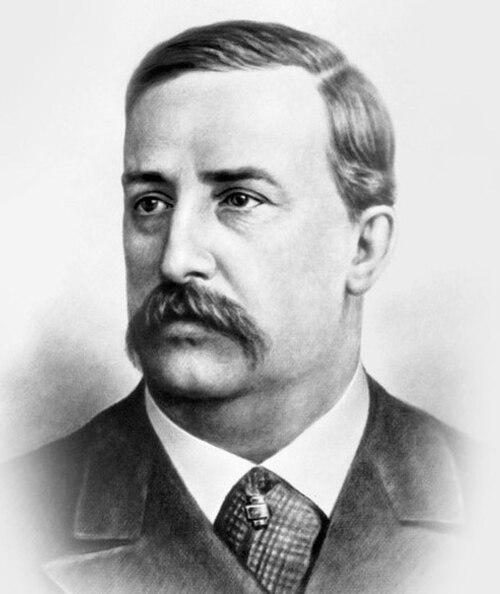
\includegraphics[width=\linewidth]{images/book3/borodin.jpg}
\end{minipage}\hspace{0.02\linewidth}%
\begin{minipage}[t]{0.18\linewidth}
\vspace{0pt}
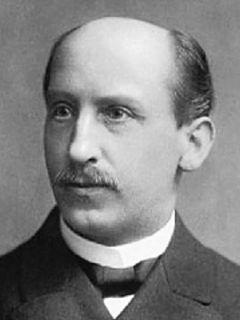
\includegraphics[width=\linewidth]{images/book3/claisen.jpg}
\end{minipage}\hfill
\begin{minipage}[t]{0.58\linewidth}
\vspace{0pt}
L'\omterm{def:b2:enolates-aldol:aldol}{aldolisation} fut décrite en 1872 par Charles-Adolphe Wurtz et, indépendamment, par Alexandre
Borodine, chimiste de Saint-Pétersbourg mieux connu aujourd'hui comme compositeur du
\textit{Prince Igor}. Ludwig Claisen étendit les condensations des composés carbonylés aux esters en
1887. (Portraits~: Borodine, auteur inconnu, domaine public~; Claisen, par Veronica.villagrasa,
CC BY-SA 4.0~; Wikimedia Commons.)
\end{minipage}
\end{history}

\begin{safety}{\ghs[5mm]{GHS02}\,\ghs[5mm]{GHS05}\,\ghs[5mm]{GHS07}}
L'éthanolate de sodium et le diisopropylamidure de lithium sont corrosifs et réagissent avec l'eau~;
les solutions de LDA sont inflammables et manipulées sous gaz inerte. Le benzaldéhyde et la
propanone sont nocifs et inflammables.
% ledger: ghs:NaOEt, ghs:LDA, ghs:benzaldehyde, ghs:acetone
\end{safety}

\section{Exercices}

\begin{exercise}[$\star$]\label{exo:b2:enolates-aldol:1}
Représenter les \omterm{def:b2:enolates-aldol:tautomerism}{tautomères} \omterm{def:b2:enolates-aldol:tautomerism}{énols} de la butanone et de la cyclohexanone.
\end{exercise}

\begin{exercise}[$\star$]\label{exo:b2:enolates-aldol:2}
Classer selon l'acidité de leur liaison \ce{C-H} la plus acide~: la propanone, la pentane-2,4-dione,
le 3-oxobutanoate d'éthyle, l'éthane.
\end{exercise}

\begin{exercise}[$\star$]\label{exo:b2:enolates-aldol:3}
Donner l'\omterm{def:b2:enolates-aldol:aldol}{aldol} et le produit de \omterm{def:b2:enolates-aldol:aldol}{crotonisation} de l'éthanal en présence d'hydroxyde de sodium.
\end{exercise}

\begin{exercise}[$\star$]\label{exo:b2:enolates-aldol:4}
Écrire la \omterm{def:b2:enolates-aldol:decarboxylation}{synthèse malonique} de l'acide hexanoïque~: quel halogénoalcane faut-il~?
\end{exercise}

\begin{exercise}[$\star\star$]\label{exo:b2:enolates-aldol:5}
Représenter les \omterm{def:b2:enolates-aldol:kinetic-enolate}{énolates cinétique} et thermodynamique de la 2-méthylcyclohexanone et les conditions
qui donnent chacun d'eux.
\end{exercise}

\begin{exercise}[$\star\star$]\label{exo:b2:enolates-aldol:6}
Donner le produit de l'aldolisation--crotonisation croisée du benzaldéhyde avec la propanone (un
équivalent de chacun) et expliquer pourquoi le benzaldéhyde ne se condense pas sur lui-même.
\end{exercise}

\begin{exercise}[$\star\star$]\label{exo:b2:enolates-aldol:7}
L'hexane-2,5-dione subit en milieu basique une aldolisation--crotonisation intramoléculaire. Quel cycle
se forme~? Expliquer le choix entre les cycles possibles.
\end{exercise}

\begin{exercise}[$\star\star$]\label{exo:b2:enolates-aldol:8}
Écrire la \omterm{def:b2:enolates-aldol:claisen}{condensation de Claisen} de l'éthanoate d'éthyle et son produit après hydrolyse acide.
\end{exercise}

\begin{exercise}[$\star\star$]\label{exo:b2:enolates-aldol:9}
Lesquels de ces composés donnent un test iodoforme positif~: propanone, pentan-3-one, éthanal, acétophénone~?
\end{exercise}

\begin{exercise}[$\star\star\star$]\label{exo:b2:enolates-aldol:10}
Écrire la cyclisation de Dieckmann de l'hexanedioate de diéthyle et la taille du cycle du produit.
\end{exercise}

\begin{exercise}[$\star\star\star$]\label{exo:b2:enolates-aldol:11}
La (\textit{R})-3-méthylpentan-2-one perd son activité optique dans l'hydroxyde de sodium dilué, mais
pas la (\textit{R})-4-méthylhexan-2-one. Expliquer.
\end{exercise}

\begin{exercise}[$\star\star\star$]\label{exo:b2:enolates-aldol:12}
Proposer une voie vers la 1,5-diphénylpenta-1,4-dién-3-one, puis vers une diénone portant deux groupes
aryle différents, et dire pourquoi la seconde est plus difficile.
\end{exercise}

\section{Problème~: la dibenzalacétone}

\begin{problem}[{Problème du week-end --- l'énolate de la propanone et le rôle du benzaldéhyde, les deux
crotonisations, le produit conjugué, et la stœchiométrie et le rendement d'une préparation}]
\label{pb:b2:enolates-aldol:1}
Préparation (données de l'exercice)~: \qty{2.1}{mL} de benzaldéhyde et \qty{0.75}{mL} de propanone sont
agités dans l'éthanol avec de l'hydroxyde de sodium aqueux~; des cristaux jaunes de
1,5-diphénylpenta-1,4-dién-3-one (dibenzalacétone) se séparent~; rendement 75~\%. Masses volumiques
(\unit{g/cm^3})~: benzaldéhyde 1.045, propanone 0.7845. Masses molaires (\unit{g/mol})~: C 12.011,
H 1.008, O 15.999.
% ledger: rho:benzaldehyde, rho:acetone, aw:C, aw:H, aw:O, ghs:dibenzalacetone

\medskip
\noindent\textbf{Partie I --- Les partenaires.}
\begin{enumerate}
  \item Quel partenaire possède des hydrogènes $\alpha$~? Combien~?
  \item Représenter l'\omterm{def:b2:enolates-aldol:enolate}{énolate} de la propanone.
  \item Pourquoi le benzaldéhyde ne peut-il pas former d'\omterm{def:b2:enolates-aldol:enolate}{énolate}~?
  \item Pourquoi la propanone réagit-elle avec le benzaldéhyde plutôt qu'avec elle-même~?
  \item Pourquoi un aldéhyde est-il un meilleur électrophile qu'une cétone~?
  \item Pourquoi l'hydroxyde suffit-il ici comme base~?
\end{enumerate}

\medskip
\noindent\textbf{Partie II --- Le mécanisme.}
\begin{enumerate}[resume]
  \item Écrire l'addition de l'\omterm{def:b2:enolates-aldol:enolate}{énolate} sur le benzaldéhyde.
  \item Écrire la déshydratation de l'\omterm{def:b2:enolates-aldol:aldol}{aldol} formé.
  \item Pourquoi la déshydratation est-elle facile ici~?
  \item Pourquoi la réaction peut-elle se produire une seconde fois~?
  \item Écrire l'équation globale.
  \item Qu'est-ce qui rend la réaction totale dans cette préparation~?
\end{enumerate}

\medskip
\noindent\textbf{Partie III --- Le produit.}
\begin{enumerate}[resume]
  \item Combien la dibenzalacétone possède-t-elle de doubles liaisons \ce{C=C}, et de quelle configuration (surtout)~?
  \item Pourquoi l'isomère (\textit{E},\textit{E}) est-il favorisé~?
  \item Compter les liaisons $\pi$ conjuguées.
  \item Pourquoi le composé est-il jaune alors que ses partenaires sont incolores~?
  \item La dibenzalacétone est-elle chirale~?
\end{enumerate}

\medskip
\noindent\textbf{Partie IV --- Stœchiométrie et rendement.}
\begin{enumerate}[resume]
  \item Calculer les masses molaires du benzaldéhyde, de la propanone et de la dibenzalacétone.
  \item Calculer les quantités des deux réactifs.
  \item Quel réactif est limitant~?
  \item Calculer la masse théorique de produit.
  \item Pourquoi un léger excès de benzaldéhyde est-il préférable à un excès de propanone~?
  \item Que donnerait un excès de propanone~?
  \item Donner la masse de dibenzalacétone obtenue avec un rendement de 75~\%.
\end{enumerate}
\end{problem}
